\chapter{Pakete}
\label{cha:pakete}
Hier werden alle verwendeten Pakete beschrieben. Diese Beschreibung
umfasst die Funktionalität und die verwendete Konfiguration der
Pakete.\\

\section{Grundlagen für die Konfiguration der Pakete}
\label{sec:basicsKonfig}
Es folgt eine Beschreibung des Paketes \textit{use-package}. Dieses
Paket wird zum Installieren und Konfigurieren aller weiteren Pakete
verwendet. Im Anschluss werden noch einige Funktionen der Sprache
Emacs Lisp beschrieben. Diese Funktionen werden für die Definition
eigener Funktionen benötigt.\\

\subsection{Use-Package}
\label{subsec:usepackage}
Das Paket \textit{use-package} verwendet die Emacs Lisp-Funktion
\textit{require}. Die Funktion \textit{require} ist in Emacs
standardmäßig implementiert. Sie erwartet einen Parameter, den Namen
eines Paketes. Die Funktion überprüft ob ein Paket mit dem Namen
bereits installiert ist. Ist dies nicht der Fall, wird das Paket
installiert. Durch die Verwendung des Paketes \textit{use-package}
wird eine einfachere Installation und Konfiguration von Paketen
ermöglicht.

Um ein gewünschtes Paket zu installieren wird erst das Kommando
{\glqq}use-package{\grqq} geschrieben, gefolgt von dem Namen des
Pakets. In dem folgendem Beispiel \ref{code:usepack}, wird das Paket
\textit{example-pack} verwendet. Es gibt einige Schlüsselwörter für
\textit{use-package}, alle beginnen mit einem
Doppelpunkt. \cite{UsePackage}\\\\ Die am häufigsten verwendeten
Schlüsselwörter folgen:
\begin{itemize}
\item \textbf{:ensure}: Folgt auf dieses Schlüsselwort der Parameter
  {\glqq}t{\grqq} für \textit{true}, so wird das Paket installiert. Es
  ist ebenfalls möglich, die Variable
  \textit{use-package-always-ensure} auf {\glqq}t{\grqq} zu setzen,
  dann wird das Verhalten von {\glqq}\textit{:ensure} t{\grqq} global
  auf alle Pakete angewendet.
\item \textbf{:init}: Nach diesem Schlüsselwort kann beliebig viel
  Emacs Lisp-Code stehen. Zu beachten ist, dass dieser Code
  \textbf{vor} dem Laden des Paketes abgearbeitet wird.
\item \textbf{:config}: Funktioniert gleich wie \textit{:init}, nur
  das dieser Code \textbf{nach} dem Laden des Paketes abgearbeitet
  wird.
\item \textbf{:bind}: Wird dazu verwendet um Tastenkombinationen
  spezifisch für dieses Paket festzulegen. Die Syntax lautet
  folgendermaßen: Erst die Tastenkombination unter doppelten
  Hochkomma, danach ein Punkt und darauf die gewünschte
  Funktionalität, mit der die Tastenkombination verknüpft
  wird. Codestück \ref{code:usepack} in Zeile fünf veranschaulicht
  dies.
\item \textbf{:map}: Dies ist eine Erweiterung für \textit{:bind}, um
  Tastenkombinationen spezifisch für einzelne Modi festlegen zu
  können. Die Syntax ist gleich wie bei \textit{:bind}, nur dass vor
  der Tastenkombination mit \textit{:map} der Modus festgelegt wird.
\item \textbf{:pin}: Mit \textit{:pin} kann direkt ausgewählt werden,
  von welchem Archiv das Paket geladen werden soll.
\item \textbf{:hook}: Dieses Schlüsselwort dient dazu, \textit{minor
  modes} an andere Modi anzuhängen. Im folgenden Beispiel wird der
  \textit{b-mode} an den \textit{a-mode} angehängt. Das bedeutet, wird
  \textit{a-mode} verwendet, so wird automatisch auch \textit{b-mode}
  aktiviert.
\item \textbf{:after}: Mit \textit{:after} kann festgelegt werden,
  welche Pakete installiert und geladen sein müssen, bevor dieses
  Paket geladen wird. Dadurch wird eine Reihenfolge für das Laden der
  Pakete definiert. Dies ist manchmal notwendig, da einige Pakete auf
  anderen aufbauen und dadurch selbstständig nicht korrekt geladen
  werden. In dieser Liste kann eine beliebige Anzahl an Paketen
  stehen.
\item \textbf{:custom}: Das Schlüsselwort \textit{:custom} wird
  verwendet, um Variable mit einem Wert zu belegen. Die Syntax lautet
  folgendermaßen: Erst der Name der Variable, danach folgt der Wert
  der zugewiesen wird, gefolgt von einem Kommentar. Codestück
  \ref{code:usepack} in Zeile neun veranschaulicht dies.
\end{itemize}

\begin{program}[h]
  \lstinputlisting[language=Lisp, firstline=1,
    lastline=10]{./code/Pakete/usepackage.el}
  \caption{\label{code:usepack}Dieses Codestück zeigt die Verwendung
    des Pakets \textit{use-package} mit {\glqq}Dummy{\grqq}-Werten.}
\end{program}

\subsection{Kommandos für die Konfiguration}
\label{subsec:kommandosKonfig}
Hier werden einige Emacs Lisp-Kommandos und Code-Zeilen aufgelistet,
welche in den Konfigurationsdateien verwendet werden:
\begin{itemize}
\item \textit{setq} : Definiert eine Variable global mit einem Wert.
\item \textit{add-hook} : Bindet zwei Objekte aneinander. Diese
  Objekte können Modi, Funktionen oder Tastenkombinationen sein.
\item \textit{defun} : Definiert eine Funktion.
\item \textit{unless} : Funktioniert wie ein if-Statement, jedoch wird
  der Code darunter ausgeführt wenn das Statement falsch
  {\glqq}nil{\grqq} ist.
\item \textit{progn} : Ermöglicht es, mehrere Funktionen
  hintereinander abzuarbeiten.
\item \textit{message} : Schreibt eine Zeichenkette in den
  {\glqq}message{\grqq} Puffer.
\item \textit{concat} : Fügt eine Zeichenkette aus mehreren kleinen
  Zeichenketten zusammen.
\item \textit{shell-command} : Führt ein Kommando in der Konsole aus.
\item \textit{file-exists-p} : Überprüft, ob eine Datei mit dem
  angegebenen Namen existiert.
\item \textit{file-directory-p} : Überprüft, ob ein Ordner mit dem
  angegebenen Namen existiert.
\item \textit{cd} : Wechselt das Verzeichnis.
\item \textit{find-file} : Öffnet eine Datei mit dem angegebenen
  Namen.
\item \textit{mkdir} : Erzeugt einen Ordner.
\end{itemize}

\section{Pakete zur Navigation}
\label{sec:navigation}
Die folgenden Pakete vereinfachen die Navigation in Emacs. Diese
vereinfachte Navigation erfolgt mit der Hilfe von Suchfunktionen
innerhalb eines Puffers. Es folgen ebenfalls Pakete für die
automatische Vervollständigung im \textit{minibuffer}.

\subsection{Avy}
\label{subsec:avy}
Das Paket \textit{Avy} wird verwendet, um an jede beliebige Position
im sichtbaren Bereich zu springen. Dies funktioniert über mehrere
Fenster, jedoch nur innerhalb eines Rahmens. \textit{Avy} stellt
folgende Funktionen zur Verfügung: \textit{avy-goto-char} und
\textit{avy-goto-char-2}. Wird die Funktionen \textit{avy-goto-char}
aufgerufen gefolgt von einem Zeichen zu dem gesprungen werden soll,
dann sucht \textit{avy} nach allen Stellen im sichtbaren Bereich, die
mit diesem Zeichen übereinstimmen. Alle Übereinstimmungen werden mit
Buchstaben markiert und durch Eintippen dieser Buchstaben springt der
Zeiger zu der gewünschten Position. Die Funktion
\textit{avy-goto-char-2} funktioniert identisch, nur dass diese
Funktion zwei Parameter nimmt, dadurch sind die Übereinstimmungen
geringer. Die folgende Grafik \ref{fig:avy} veranschaulicht diese
Beschreibung. In der Abbildung wird dieser Text zur Beschreibung des
Paketes \textit{avy} angezeigt.  Zum Springen wird die Funktion
\textit{avy-goto-char-2} verwendet. Gesprungen werden soll zu dem
vorletzten {\glqq}Avy{\grqq} im angezeigtem Fenster. In der Abbildung
sind alle {\glqq}av{\grqq} mit Buchstaben markiert. Um zu dem
gewünschten Zeichen zu springen müssen die Buchstaben {\glqq}l{\grqq}
und {\glqq}h{\grqq} eingetippt werden. \cite{Avy}

\begin{figure}[h]
  \centering
  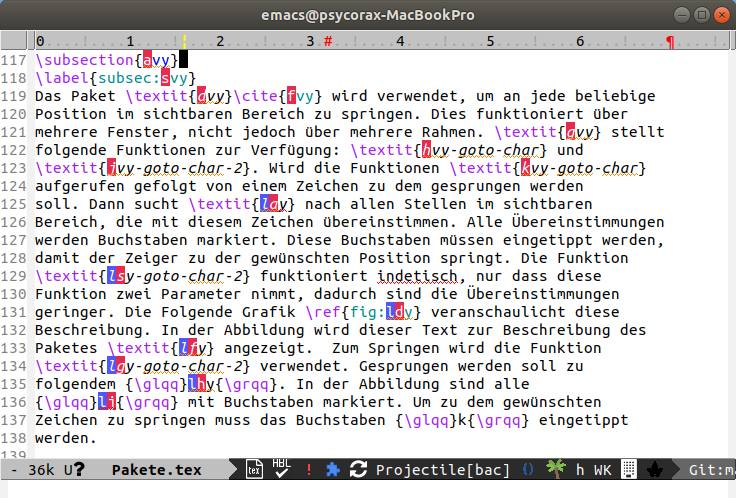
\includegraphics[width=.95\textwidth]{./images/Pakete/avy.png}
  \caption{\label{fig:avy} Das Paket \textit{avy} hat alle gefundenen
    {\glqq}av{\grqq}-Zeichenketten markiert und vorübergehend mit
    anderen Buchstaben überschrieben. Über diese temporären Buchstaben
    ist die gewünschte Zeichenkette erreichbar.}
\end{figure}

\subsubsection{Verwendete Kommandos und Tastenkombinationen}
Das Kommando \textit{avy-goto-char-2} wird an die Tastenkombination
\textbf{M-s} gebunden.\\

\subsection{Ivy}
\label{subsec:ivy}
\textit{Ivy} ermöglicht eine Vervollständigung für Kommandos im
\textit{minibuffer}. Einige dieser Kommandos sind \textit{find-file},
\textit{M-x} und \textit{switch-buffer}. Wird \textit{find-file}
ausgeführt, so zeigt \textit{Ivy} die Dateien und Ordner in dem
aktuellen Verzeichnis an. Wird etwas eingetippt, so werden nur noch
Dateien und Ordner angezeigt, die diese eingetippte Zeichenkette
enthalten. Das Leerzeichen wird als Wildcard interpretiert. Wird zum
Beispiel {\glqq}<SPACE>.tex{\grqq} eingetippt so werden nur noch
tex-Dateien angezeigt. Dies funktioniert bei dem Befehl \textit{M-x}
auch für Funktionen. Die Grafik \ref{fig:ivy} veranschaulicht diese
Beschreibung. In der Abbildung wurde zu einem
\textit{Latex}-Verzeichnis navigiert. In diesem Verzeichnis wird nach
allen Dateien und Ordnern gesucht, welche die Zeichenkette
{\glqq}tex{\grqq} enthalten. \cite{Ivy}\\

\subsubsection{Verwendete Kommandos und Tastenkombinationen}
Das Kommando \textit{ivy-switch-buffer} wird in der
Konfigurationsdatei, welche im Zuge der Arbeit entstanden ist, an die
Tastenkombination \textbf{C-x b} gebunden. Außerdem wird \textit{ivy}
global aktiviert.\\

\begin{figure}[h]
  \centering
  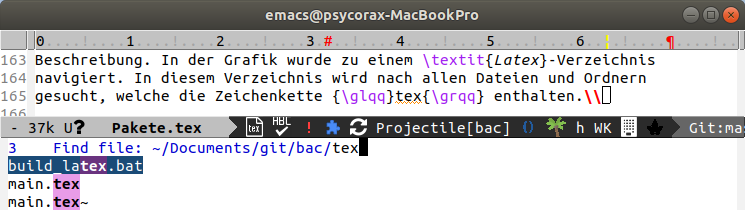
\includegraphics[width=.95\textwidth]{./images/Pakete/ivy.png}
  \caption{\label{fig:ivy} Die verbesserte Suche mit dem Paket
    \textit{ivy} wird in dieser Abbildung dargestellt.}
\end{figure}

\subsection{Swiper}
\label{subsec:swiper}
\textit{Swiper} ist eine Alternative zu
       {\glqq}isearch{\grqq}. \textit{Isearch} ist in Emacs
       standardmäßig enthalten. Das Paket \textit{swiper} verwendet
       \textit{Ivy} um eine Übersicht der Übereinstimmungen im
       \textit{minibuffer} anzuzeigen. Zwischen diesen
       Übereinstimmungen kann mit den Pfeiltasten gesprungen
       werden. Das Leerzeichen dient auch hier als
       Wildcard. \cite{Swiper}\\

\subsubsection{Verwendete Kommandos und Tastenkombinationen}
Das Kommando \textit{swiper} wird in der Konfigurationsdatei, welche
im Zuge der Arbeit entstanden ist, an die Tastenkombinationen
\textbf{C-s} und \textbf{C-r} gebunden.\\

\subsection{Counsel}
\label{subsec:counsel}
\textit{Counsel} erweitert das Paket \textit{Ivy}. Diese Erweiterungen
umfassen das Ersetzen einiger Kommandos. So wird zum Beispiel
\textit{find-file} mit \textit{counsel-find-file} ersetzt. Dadurch
wird dieses Kommando erweitert. Eine solche Erweiterung ist, dass mit
der {\glqq}Del-Taste{\grqq} um ein Verzeichnis zurück gesprungen
wird. Dies erspart das Tippen von {\glqq}../{\grqq}. Ebenso sind
mehrere Optionen verfügbar, welche das Öffnen der Dateien betreffen,
wenn im \textit{minibuffer} die Tastenkombination \textbf{M-o}
gedrückt wird. Eine weiter erwähnenswerte Funktion ist
\textit{counsel-yank-pop}. Diese Funktion ersetzt die Funktion
\textit{yank-pop}, welche standardmäßig einen {\glqq}kill
ring{\grqq}\footnote{\url{https://www.gnu.org/software/emacs/manual/html_node/emacs/Earlier-Kills.html}}
enthält. In diesem \textit{kill ring} werden früher kopierte
Zeichenketten {\glqq}kills{\grqq} abgespeichert. Durch die Verwendung
der Funktion \textit{counsel-yank-pop} wird im \textit{minibuffer}
eine Vorschau dieser Zeichenketten angezeigt. Mit den Pfeiltasten kann
durch diese gespeicherten {\glqq}kills{\grqq} navigiert
werden. \cite{Counsel}\\

\subsubsection{Verwendete Kommandos und Tastenkombinationen}
Folgende Funktionen werden durch die \textit{counsel}-Funktionen in
der Konfigurationsdatei, welche im Zuge der Arbeit entstanden ist,
ersetzt:
\begin{itemize}
\item \textbf{M-x} : \textit{counsel-M-x}
\item \textbf{C-x C-f} : \textit{counsel-find-file}
\item \textbf{M-y} : \textit{counsel-yank-pop}
\end{itemize}

\section{Pakete für die automatische Vervollständigung}
\label{sec:autocomplete}
Für Emacs gibt es zwei {\glqq}große{\grqq} Pakete für die automatische
Vervollständigung von Zeichenketten. Diese sind \textit{auto-complete}
(siehe Abschnitt \ref{subsec:ac}) und \textit{company} (siehe
Abschnitt \ref{subsec:company}). Die Unterschiede sind sehr fein. In
dieser Arbeit werden beide Pakete parallel
verwendet. \textit{Auto-complete} wird für den \textit{org-mode}
verwendet, da es ein zusätzliches Paket für \textit{auto-complete}
gibt, welches spezifisch für den \textit{org-mode} ist. Dieses Paket
hat den Namen \textit{org-ac} (siehe Abschnitt
\ref{subsubsec:orgac}). Es bietet eine verbesserte Vervollständigung
für die Makros des \textit{org-modes}. Für \textit{company} gibt es
kein vergleichbares zusätzliches Paket. \textit{Company} wird hingegen
für alle anderen \textit{major modes} verwendet. Der Grund dafür ist,
dass \textit{auto-complete} beim Ausführen der Standardkonfiguration,
automatisch in jeden \textit{major mode} eingehängt wird. So müsste
\textit{auto-complete} explizit aus jedem \textit{major mode}, in dem
es nicht gebraucht wird, wieder ausgehängt werden. \textit{Company}
ist in Verbindung mit \textit{irony} (siehe Abschnitt
\ref{subsec:irony}) für C++ nur schwer zu umgehen. Auch \textit{Elpy}
(siehe Abschnitt \ref{subsec:elpy}) welches ein Paket für Python ist,
verwendet ebenfalls \textit{company}.\\

\subsection{Auto-Complete}
\label{subsec:ac}
Um \textit{auto-complete} zu verwenden, kann das Kommando
\textit{ac-config-default} aufgerufen werden. Dadurch wird
\textit{auto-complete} für alle \textit{major modes} konfiguriert und
eingehängt. Wird \textit{auto-complete} in einem bestimmten Modus
nicht benötigt, so muss dies explizit eingestellt werden. Wird
\textit{auto-complete} in Verbindung mit \textit{flyspell} (siehe
Abschnitt \ref{subsec:flyspell}) verwendet, so muss das Kommando
\textit{ac-flyspell-workaround} ausgeführt werden. Ansonsten
aktualisieren sich möglichen Vervollständigung nicht
mehr. \cite{AutoComplete}\\

\subsubsection{Org-Ac}
\label{subsubsec:orgac}
\textit{Org-ac} ist eine Vervollständigung für die Makros im
\textit{org-mode}. Ein Vorteil dieses Paketes ist zum Beispiel, dass
bei dem Makro \textit{\#+AUTHOR:} auch automatisch der Name
hinzugefügt wird. Bei \textit{\#+DATE:} wird automatisch das heutige
Datum angefügt. Zum Konfigurieren muss das Kommando nach dem Laden des
Paketes \textit{org-ac/config-default} ausgeführt werden. Dies bindet
den \textit{auto-complete-mode} auch direkt an den
\textit{org-mode}. \cite{OrgAC}\\

\subsection{Company}
\label{subsec:company}
\textit{Company} konfiguriert sich bei der Installation selbst mit den
Standardeinstellungen, hängt sich jedoch nicht in \textit{major modes}
selbstständig ein. Es unterstützt eine Vielzahl an Unterbauten
({\glqq}back-ends{\grqq}). Folgende \textit{back-ends} werden genutzt:
\begin{itemize}
\item CAPF : Unterstützt Vervollständigung von Strukturen in allen
  Programmiersprachen.
\item Elisp : Für die Programmiersprache Emacs Lisp.
\item Clang : Für die Programmiersprache C und C++.
\item ISpell : Für das Paket \textit{flyspell} (siehe Abschnitt
  \ref{subsec:flyspell}).
\item CMake : Für den \textit{cmake-mode} welcher zum Erstellen von
  CMake-Dateien verwendet wird.
\item Yasnippet : Für das Paket \textit{yasnippet} (siehe Abschnitt
  \ref{subsec:yasnippet}).
\item ctags : Ein System zum Taggen (siehe Abschnitt
  \ref{subsec:ctags}).
\item files : Unterstützt Ordner und Dateien, wenn diese in einer
  Datei angegeben werden.
\item keywords : Schlüsselwörter in allen Modi.\\
\end{itemize}
Bei der Konfiguration gibt es einen wichtigen Parameter
(\textit{company-idle-delay}). Wird diese Variable auf null gesetzt,
so vervollständigt \textit{company} ohne Verzögerung. Dies kann bei
leistungsschwachen Rechnern zu Problemen führen. Sollten Probleme
durch \textit{company} auftreten, kann der Wert auf eins abgeändert
werden. Eine weitere verwendete Variable ist
\textit{company-minimum-prefix-length}. Diese bestimmt, ab wie vielen
Zeichen eine Vervollständigung erfolgen soll. \cite{Company}\\

\section{Sonstige Pakete}
\label{sec:misc}
Hier folgen grundlegende Pakete, welche die Benutzung von Emacs
einfacher oder effizienter machen.\\

\subsection{Acewindow}
\label{subsec:acewindow}
Das Paket \textit{ace-window} vereinfacht die Navigation zwischen
Rahmen und Fenstern. Das Kommando \textit{ace-window} ersetzt das
Kommando \textit{other-window}. Das in Emacs standardmäßig enthaltene
Kommando \textit{other-window} wechselt zu Fenstern innerhalb eines
Rahmens in einer definierten Reihenfolge. \textit{Ace-window}
erweitert dies, indem die Fenster in dieser Reihenfolge nummeriert
werden. Sind mehr als zwei Fenster offen, werden bei dem Ausführen des
Kommandos der Inhalt der Fenster {\glqq}schwächer{\grqq}
dargestellt. Im jeweils \textit{oberen linken} Rand befindet sich die
Nummer des Fensters. Über diese Nummer ist nun das jeweilige Fenster
erreichbar. Mit \textit{ace-window} kann auch zu den Fenstern
unterschiedlicher Rahmen gesprungen werden. Die folgende Grafik
\ref{fig:acewindow} veranschaulicht dies. \cite{AceWindow}

\begin{figure}[h]
  \centering
  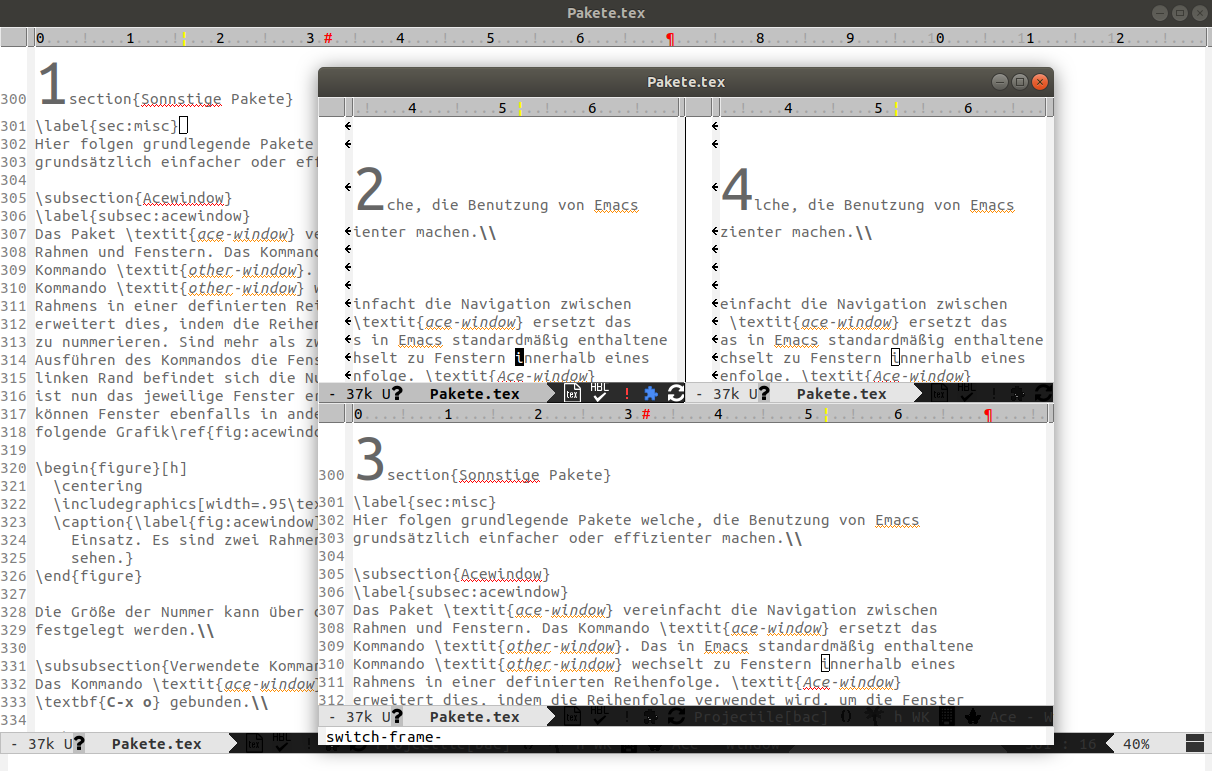
\includegraphics[width=.95\textwidth]{./images/Pakete/acewindow.png}
  \caption{\label{fig:acewindow} Das Paket \textit{ace-window} im
    Einsatz. Es sind zwei Rahmen mit insgesamt vier Fenstern zu
    sehen.}
\end{figure}

Die Größe der dargestellten Nummer kann über den Parameter
\textit{:height} festgelegt werden. Für die Grafik \ref{fig:acewindow}
wurde für \textit{:height} der Wert 4.0 verwendet.\\

\subsubsection{Verwendete Kommandos und Tastenkombinationen}
Das Kommando \textit{ace-window} wird in der Konfigurationsdatei,
welche im Zuge der Arbeit entstanden ist, an die Tastenkombination
\textbf{C-x o} gebunden.\\

\subsection{Try}
\label{subsec:try}
Das Paket \textit{try} wird verwendet, um andere Pakete testen zu
können. Sollte ein neues Paket ausprobiert werden, dann wird einfach
\texttt{M-x try} ausgeführt und in den \textit{minibuffer} wird der
Namen des neuen Pakets getippt. Dadurch wird das Paket für die
aktuelle Sitzung installiert. Bei einem Neustart von Emacs ist das
Paket nicht mehr vorhanden. \cite{Try}\\

\subsection{Which-Key}
\label{subsec:whichkey}
Das Paket \textit{which-key} ist sehr hilfreich für
Emacs-Neulinge. Wird eine Tastenkombination eingetippt welche eine
weitere Eingabe erfordert, so erscheint ein Fenster mit den möglichen
Kombinationen. In der folgenden Abbildung \ref{fig:whichkey} wurde die
Tastenkombination \textbf{C-x} eingetippt. Die Grafik zeigt das
geöffnete \textit{which-key}-Fenster. In dem Fenster sind alle
möglichen Tastenkombinationen zu sehen, inklusive der
Beschreibungen. Diese Beschreibungen erläutern, welche Funktion hinter
den Tastenkombinationen steckt. Mit jeweils \textbf{C-h n} und
\textbf{C-h p} kann durch die Seiten {\glqq}geblättert{\grqq}
werden. Die Zeit nach der dieses \textit{which-key}-Fenster erscheinen
soll, kann über die Variable \textit{which-key-idle-delay} definiert
werden. \cite{WhichKey}\\

\begin{figure}[h]
  \centering
  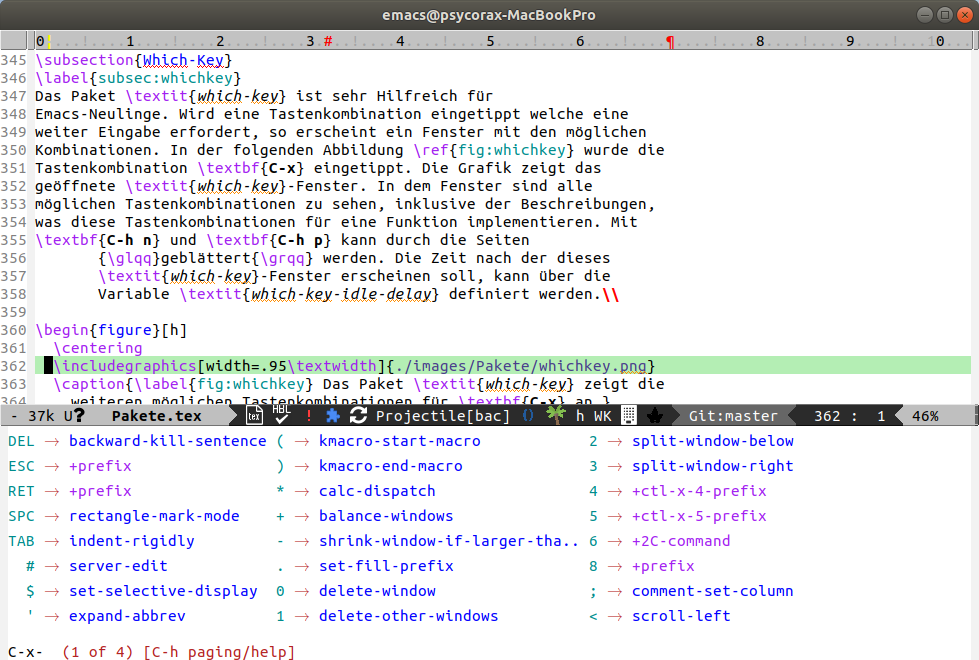
\includegraphics[width=.95\textwidth]{./images/Pakete/whichkey.png}
  \caption{\label{fig:whichkey} Das Paket \textit{which-key} zeigt die
    weiteren möglichen Tastenkombinationen für \textbf{C-x} an.}
\end{figure}

\subsubsection{Verwendete Konfigurationen}
Die Zeit bis das Fenster auftaucht wird in der Konfigurationsdatei,
welche im Zuge der Arbeit entstanden ist, auf eine Sekunde gesetzt.\\

\subsection{Hungry-Delete}
\label{subsec:hungrydelete}
\textit{Hungry-delete} ist ein Paket, mit dem alle aufeinander
folgenden Leerzeichen auf einmal gelöscht werden können. Standardmäßig
ist die Funktionalität \textit{hungry-delete} nur im
\textit{cc-mode}\footnote{\url{https://www.gnu.org/software/emacs/manual/html_mono/ccmode.html}}
implementiert. Das Paket \textit{Hungry-delete} lagert diese
Funktionalität in einen \textit{minor mode} aus. Dadurch kann
\textit{hungry-delete} in allen beliebigen \textit{major modes}
verwendet werden. \cite{HungryDelete}\\

\subsubsection{Verwendete Konfigurationen}
Der \textit{hungry-delete}-Modus wird global aktiviert.\\

\subsection{Expand-Region}
\label{subsec:expandregion}
Das Paket \textit{expand-region} ermöglicht ein schnelles Markieren
von Text. Mit dem ersten Ausführen der Funktion
\textit{er/expand-region}, wird das Wort auf dem sich der Zeiger
befindet markiert. Nun kann mit den folgenden drei Tasten die Region
angepasst werden:
\begin{itemize}
\item \textbf{+} : Erweitert die Region.
\item \textbf{-} : Geht eine Erweiterung zurück.
\item \textbf{0} : Bricht die Funktion ab.
\end{itemize}
Regionen sind anfangs durch das Wort definiert. Weitere Abgrenzungen
der Regionen erfolgt durch Klammern, Hochkomma und
Absätze. \cite{ExpandRegion}\\

\subsubsection{Verwendete Kommandos und Tastenkombinationen}
Die Funktion \textit{er/expand-region} wird an Tastenkombination
\textbf{C-+} gebunden.

\subsection{Multiple-Cursors}
\label{subsec:multiplecursors}
Das Paket \textit{multiple-cursors} ermöglicht es, mehrerer Zeiger auf
einmal steuern zu können. Dadurch kann Text an mehreren Stellen zur
selben Zeit editiert werden. Auf die einzelnen Cursor können auch
Makros angewendet werden. Die wichtigsten Funktionen zum Setzen der
Zeiger sind:
\begin{itemize}
\item \textit{mc/mark-next-like-this} : Es wird eine Übereinstimmung
  vor der markierten Zeichenkette gesucht und mit einem zusätzlichen
  Zeiger markiert.
\item \textit{mc/mark-previous-like-this} : Es wird eine
  Übereinstimmung nach der markierten Zeichenkette gesucht und mit
  einem zusätzlichen Zeiger markiert.
\item \textit{mc/mark-all-like-this} : Es werden alle
  Übereinstimmungen mit der markierten Zeichenkette gesucht und mit
  einem zusätzlichen Zeiger markiert.
\end{itemize}
Sind mehrere Zeiger vorhanden, führen alle Zeiger das selbe
aus. \cite{MultipleCursors}\\\\ Auf der Webseite \textit{Emacs
  Rocks!}\footnote{\url{http://emacsrocks.com/}} wird in dem Video
\textit{Epsiode 13:
  multiple-cursors}\footnote{\url{http://emacsrocks.com/e13.html}} das
Potential von \textit{multiple-cursors} sehr gut veranschaulicht.\\

\subsubsection{Verwendete Kommandos und Tastenkombinationen}
Die Funktionen sind in der Konfiguration mit folgenden
Tastenkombinationen verknüpft:
\begin{itemize}
\item \textbf{C->} : \textit{mc/mark-next-like-this}
\item \textbf{C-<} : \textit{mc/mark-previous-like-this}
\item \textbf{C-M-<} : \textit{mc/mark-all-like-this}
\end{itemize}

\subsection{Flyspell}
\label{subsec:flyspell}
\textit{Flyspell} ist ein integriertes Paket in Emacs und muss nicht
explizit installiert werden. Das Paket dient der Rechtschreibprüfung.
Dadurch können einfache Tippfehler vermieden werden. Eine Überprüfung
der Grammatik ist mit diesem Paket nicht möglich. \cite{Flyspell}\\

\subsubsection{Verwendete Konfigurationen}
Es wird eine Funktion verwendet, welche zwischen den Wörterbüchern
Deutsch und Englisch wechselt. Diese Funktion
\textit{fd-switch-dictionary} wird an die Taste \textbf{<F9>}
gebunden.\\

\subsection{Undo-Tree}
\label{subsec:undotree}
Die Rückgängig- und Wiederholen-Funktion in Emacs sind nicht sehr
leicht Überschaubar, da diese einen kompletten Baum aufbauen
können. Das Paket \textit{undo-tree} implementiert eine grafische
Oberfläche. Dadurch ist es einfacher, den Veränderungen zu folgen,
wenn diese wirr verzweigt sind. Die {\glqq}o{\grqq} stellen die Knoten
dar und das {\glqq}x{\grqq} die aktuelle Position. Ist der
\textit{undo-tree} geöffnet, so kann mit Tasten noch weitere
Funktionalität eingeschaltet werden. Diese möglichen Tasten sind:
\begin{itemize}
\item \textbf{t} : Aktiviert Zeitpunkte, wann die einzelnen Knoten das
  letzte mal besucht wurden.
\item \textbf{d} : Zeigt die Unterschiede der einzelnen Knoten in
  einem zusätzlichen Fenster.
\item \textbf{q} : Verlässt die grafische Anzeige \textit{undo-tree}
  an dem momentan befindlichem Knoten.
\end{itemize}
Die folgende Abbildung \ref{fig:undotree} zeigt das Fenster des
\textit{undo-trees}. \cite{UndoTree}

\begin{figure}[h]
  \centering
  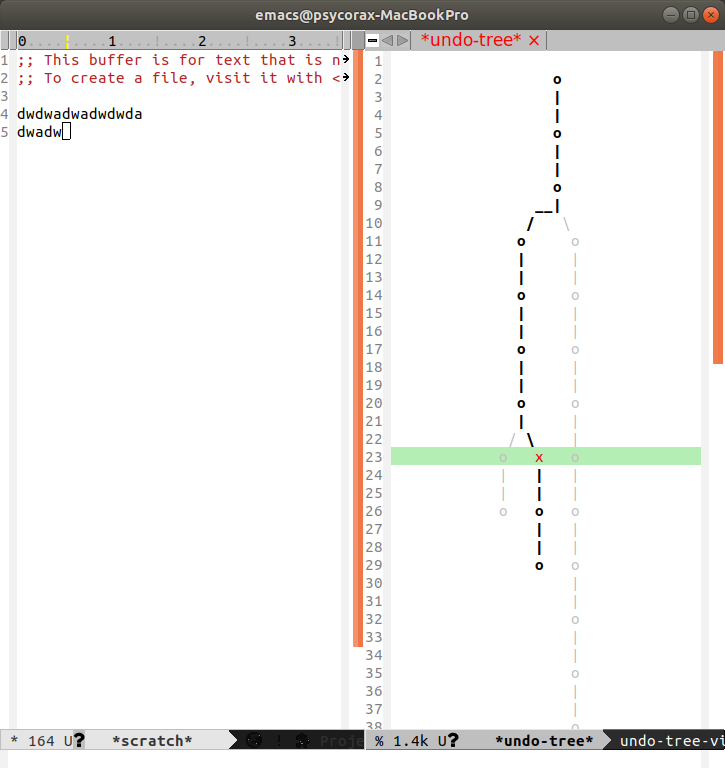
\includegraphics[width=.95\textwidth]{./images/Pakete/undotree.png}
  \caption{\label{fig:undotree} Die Abbildung zeigt das Fenster des
    Paketes \textit{undo-tree}. Es ist keine zusätzliche
    Funktionalität eingeschaltet.}
\end{figure}

\subsubsection{Verwendete Konfigurationen}
Der \textit{undo-tree-mode} wird global aktiviert. Dadurch wird das
\textit{undo-tree}-Fenster bei einem einfach {\glqq}Rückgängig{\grqq}
geöffnet. {\glqq}Rückgängig{\grqq} ist in Emacs standardmäßig an
Tastenkombination \textbf{C-x u} gebunden.\\

\subsection{Smartparens}
\label{subsec:smartparens}
Das Paket \textit{smartparens} fügt bei der Erzeugung einer öffnenden
Klammer sofort auch die schließende Klammer ein. Dabei wird der Zeiger
zwischen den Klammern behalten. Ist etwas markiert, so wird der
markierte Bereich mit Klammern eingeschlossen. Dies funktioniert
ebenso mit Hochkomma. \cite{Smartparens}\\

\subsection{Hydra}
\label{subsec:hydra}
Das Paket \textit{hydra} vereinfacht die Verwendung von
Tastenkombinationen. Es funktioniert in der Verwendung ähnlich wie
\textit{which-key} (siehe Abschnitt \ref{subsec:whichkey}). Eine
\textit{hydra} ist eine Funktionalität, welche mittels Tastendruck
weitere Funktionen über Tastenkombinationen veranschaulicht darstellt
und ermöglicht. Dadurch müssen nicht alle Tastenkombinationen
auswendig gelernt werden. Eine \textit{hydra} wird auf eine
Tastenkombination gebunden, welche beim Ausführen dieser
Tastenkombination in einem Fenster erscheint. In der jeweiligen
\textit{hydra} ist definiert, auf welche Tasten welche Funktionalität
folgt. In dem folgendem Codestück \ref{code:hydra} ist die Definition
einer \textit{hydra} zu sehen. Ganz oben in der ersten Zeile wird der
\textit{hydra} ein Name zugewiesen. Darunter in den Zeilen zwei bis
fünf wird exakt definiert, wie die Darstellung der \textit{hydra} beim
Aufruf aussehen soll. Dies ist in der Abbildung \ref{fig:hydra} zu
sehen. In den Zeilen sechs bis elf werden die einzelnen Tasten der
Funktionalität zugewiesen. Am Ende des Codestücks in den Zeilen 14 bis
15 wird diese \textit{hydra} einer Taste zugewiesen. \cite{Hydra}\\

\begin{program}[h]
  \lstinputlisting[language=Lisp, firstline=1,
    lastline=15]{./code/Pakete/hydra.el}
  \caption{\label{code:hydra}Dieses Codestück zeigt die Definition
    einer \textit{hydra} für den \textit{vhdl-mode}.}
\end{program}

\begin{figure}[h]
  \centering
  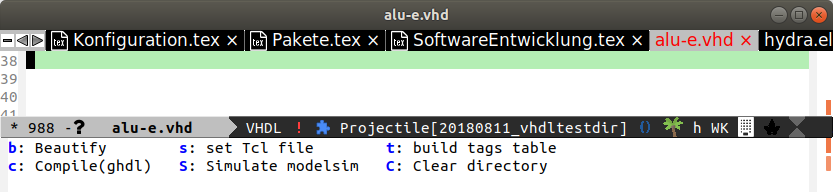
\includegraphics[width=.95\textwidth]{./images/Pakete/hydra.png}
  \caption{\label{fig:hydra} Die geöffnete \textit{hydra} für den
    \textit{vhdl-mode}.}
\end{figure}

\subsubsection{Verwendete Konfigurationen}
In dieser Arbeit wurde fallweise eine \textit{hydra} pro \textit{major
  mode} definiert. Dadurch konnten alle \textit{hydras} der Taste
\textbf{<F8>} zugewiesen werden. So wird bei dem Drücken der F8-Taste
eine für den \textit{major mode} spezifische \textit{hydra}
geöffnet. In der Arbeit wurden \textit{hydras} für folgende
\textit{major modes} festgelegt:
\begin{itemize}
\item org
\item C
\item C++
\item Python
\item VHDL
\end{itemize}
Zu beachten ist, dass \textit{treemacs} (siehe Abschnitt
\ref{subsec:treemacs}) eine eigene Hydra definiert.\\

\subsection{Projectile}
\label{subsec:projectile}
\textit{Projectile} wird zum Erkennen und Festlegen von Projekten
verwendet. Durch \textit{projectile} werden Verzeichnisse welche mit
Versionsverwaltungssystemen verwaltet werden, automatisch als Projekt
erkannt. Zusätzlich erkennt \textit{projectile} Verzeichnisse als
Projekte, wenn eine leere Datei mit dem Namen
{\glqq}.projectile{\grqq} vorhanden ist. Durch die Definition von
Projekten, werden zusätzliche Funktionen für die Suche
bereitgestellt. Diese zusätzlichen Such-Funktionen beschränken sich
auf das aktuelle Projekt. Dadurch kann Zeit gespart
werden. \cite{Projectile}\\

\subsubsection{Verwendete Konfigurationen}
Der \textit{projectile-mode} wird global eingeschaltet. Die
automatische Vervollständigung der \textit{projectile}-Funktionen wird
durch \textit{ivy} (siehe Abschnitt \ref{subsec:ivy}) durchgeführt.\\

\subsection{Magit}
\label{subsec:magit}
Das Paket \textit{magit} implementiert eine komplette Oberfläche für
\textit{Git}. Alle gängigen Kommandos für \textit{git} können mit
diesem Paket einfach ausgeführt werden. Es ist eine Kombination aus
Konsole und grafischer Oberfläche. Die Anzeige erfolgt grafisch, es
kann jedoch alles mit Tastenkombinationen gesteuert werden. Alle
möglichen Tastenkombinationen können mit der Eingabe eines
Fragezeichens angezeigt werden. Dadurch sind alle Kommandos sehr
übersichtlich dargestellt und müssen nicht auswendig gelernt
werden. Dieses Paket ist sowohl für Anfänger als auch erfahrene
\textit{Git}-Benutzer geeignet. \cite{Magit}\\\\ Für eine Einführung
in \textit{magit} wird der folgende Link \cite{MagitGuide}
empfohlen.\\

\subsubsection{Verwendete Konfigurationen}
Das \textit{magit}-Fenster kann mit der Tastenkombination \textbf{C-x
  g} aufgerufen werden. Es werden spezifische Farben für die
Markierungen des Hintergrunds festgelegt. Da sich diese Farben mit dem
in dieser Arbeit verwendeten Farbschema (siehe Abschnitt
\ref{subsec:themes}) besser vertragen.\\

\section{Pakete für grafische Elemente}
\label{sec:gui}
Die folgenden Pakete modifizieren die grafische Oberfläche von
Emacs. Einige dieser Pakete unterstützen auch die Verwendung der
Maus. Im Anhang auf den Seiten \pageref{fig:nogui} und
\pageref{fig:gui} befinden sich zwei Abbildungen von
Emacs-Rahmen. Einmal mit und einmal ohne grafische Elemente. Es wird
bei beiden das Farbschema {\glqq}zenburn{\grqq} (siehe Abschnitt
\ref{subsec:themes}) verwendet.\\

\subsection{Themes}
\label{subsec:themes}
In Emacs sind standardmäßig {\glqq}Farbschemas{\grqq}
(\textit{themes}) enthalten. Diese können einfach mit dem Befehl
\texttt{M-x load-theme} ausgewählt werden. Es gibt auch externe
\textit{themes}, welche von der \textit{Community} zur Verfügung
gestellt werden. Diese werden auf unterschiedlichen
Webseiten\footnote{\url{https://pawelbx.github.io/emacs-theme-gallery/}}
gesammelt. Die meisten \textit{themes} von diesen Seiten können auch
direkt von \textit{melpa} (siehe Abschnitt \ref{sec:paketebasics})
installiert werden.\\

\subsubsection{Verwendete Konfigurationen}
In dieser Arbeit sind zwei externe \textit{themes} konfiguriert. Das
\textit{theme}
       {\glqq}Zenburn\footnote{\url{https://github.com/bbatsov/zenburn-emacs}}{\grqq}
       und das \textit{theme}
       {\glqq}hemisu-dark\footnote{\url{https://github.com/andrzejsliwa/hemisu-theme}}{\grqq}.\\

\subsection{Powerline}
\label{subsec:powerline}
Das Paket \textit{powerline} reorganisiert die \textit{mode line}
(siehe Abschnitt \ref{sec:emacsstart}). Dadurch wird diese Leiste
übersichtlicher dargestellt. Es werden fünf unterschiedliche Schemata
zur Verfügung gestellt nach welchen die Leiste angeordnet werden
kann. Dieses Paket ist im Anhang auf Seite \pageref{fig:gui} in der
Abbildung \ref{fig:gui} im Bereich {\glqq}A{\grqq} zu
sehen. \cite{Powerline}\\

\subsection{Mode-Icons}
\label{subsec:modeicons}
\textit{Mode-icons} ersetzt die Namen der Modi durch Icons in der
\textit{mode line} (siehe Abschnitt \ref{sec:emacsstart}). Die Icons
benötigen viel weniger Platz als die ausgeschriebenen Namen der
Modi. Dadurch ist mehr Platz in der\textit{mode line}, wodurch diese
übersichtlicher erscheint. Werden Modi nicht von dem Paket
\textit{mode-icons} unterstützt, so wird dieser Modus ausgeschrieben
dargestellt. Dieses Paket ist im Anhang auf Seite \pageref{fig:gui} in
der Abbildung \ref{fig:gui} im Bereich {\glqq}B{\grqq} zu
sehen. \cite{ModeIcons}\\

\subsection{Tabbar-Ruler}
\label{subsec:tabbarruler}
Dieses Paket benutzt die Pakete \textit{powerline} (siehe Abschnitt
\ref{subsec:powerline}), \textit{mode-icons} (siehe Abschnitt
\ref{subsec:modeicons}) und \textit{tabbar} (siehe Abschnitt
\ref{subsubsec:tabbar}). Durch das Paket \textit{tabbar-ruler} werden
die Menüleiste, die Symbolleiste und die Leiste mit den Tabs am oberen
Ende des Rahmens versteckt. Wird innerhalb eines Puffers gearbeitet,
so erscheint am oberen Rand ein {\glqq}Lineal{\grqq}. Dieses Lineal
gibt die horizontale Position des Zeigers wieder. Wird der Mauszeiger
an das obere Ende des Rahmen bewegt, so verschwindet das
{\glqq}Lineal{\glqq} und die versteckten Leisten erscheinen. Des
weiteren werden neben den Namen der Tabs die zugehörigen Symbole
angezeigt. Die aufgeklappte Menüleiste und Tableiste ist im Anhang auf
Seite \pageref{fig:gui} in der Abbildung \ref{fig:gui} im Bereich
{\glqq}C{\grqq} zu sehen. \cite{TabbarRuler}\\

\subsubsection{Verwendete Konfigurationen}
In dieser Arbeit ist \textit{tabbar-ruler} folgendermaßen
konfiguriert. Die Tableiste, das Lineal, die Menüleiste und die
Scrollleiste sind aktiviert. Die Symbolleiste ist deaktiviert.\\

\subsubsection{Tabbar}
\label{subsubsec:tabbar}
Dieses Paket erzeugt am oberen Ende des Fensters eine Leiste mit
Tabs. Diese Tabs repräsentieren die offenen Puffer. \cite{Tabbar}\\

\subsection{Org-Bullets}
\label{subsec:orgbullets}
Das Paket \textit{org-bullets} stellt im \textit{org-mode} die
Aufzählungszeichen durch ein beliebiges Zeichen der
\textit{UTF-8-Codetabelle}\footnote{\url{https://www.utf8-zeichentabelle.de/unicode-utf8-table.pl}}
dar. Dadurch sind die Aufzählungen übersichtlicher. Es können auch
mehrere Zeichen definiert werden, damit werden für die
unterschiedlichen Hierarchien unterschiedliche Zeichen
verwendet. Dieses Paket ist im Anhang auf Seite \pageref{fig:gui} in
der Abbildung \ref{fig:gui} im Bereich {\glqq}D{\grqq} zu
sehen. \cite{OrgBullets}\\

\subsubsection{Verwendete Konfigurationen}
Der \textit{org-bullets-mode} wird an den \textit{org-mode}
angehängt. Als Aufzählungszeichen werden Bindestriche {\glqq}-{\grqq}
verwendet, weil Latex mit der Darstellung einiger
\textit{utf-8}-Zeichen Probleme hat.\\

\subsection{Treemacs}
\label{subsec:treemacs}
Dieses Paket implementiert einen grafischen Dateimanager in Emacs. Es
können einzelne Projekte hinzugefügt und entfernt werden. Innerhalb
von Projekten können Dateien umbenannt, erstellt oder gelöscht
werden. Dieser Dateimanager kann auch mit der Maus bedient
werden. Dieses Paket ist im Anhang auf Seite \pageref{fig:gui} in der
Abbildung \ref{fig:gui} im Bereich {\glqq}E{\grqq} zu
sehen. \cite{Treemacs}\\

\subsubsection{Verwendete Konfigurationen}
Es wird die empfohlene
Konfiguration\footnote{\url{https://github.com/Alexander-Miller/treemacs\#installation}}
verwendet. Zusätzlich wird das Öffnen und Schließen von Ordnern und
Dateien von einem Doppelklick mit der Maus, auf einen einfachen Klick
abgeändert\footnote{\url{https://github.com/Alexander-Miller/treemacs\#mouse-interface}}.

\section{Pakete zum Programmieren}
Die folgenden Pakete unterstützen den Benutzer beim Implementieren von
Software in unterschiedlichsten Sprachen.\\

\subsection{Ag}
\label{subsec:ag}
Das Paket \textit{ag} wird zur dateiübergreifenden Suche verwendet. Es
verwendet das Programm
\textit{silversearcher}\footnote{\url{https://github.com/ggreer/the_silver_searcher}}
zur Suche. In der Fußzeile ist ein
Link\footnote{\url{https://github.com/ggreer/the_silver_searcher\#installing}}
zu finden, wo beschrieben wird wie \textit{silversearcher} auf den
gängigsten Betriebssystemen installiert werden kann. \cite{Ag}\\

\subsubsection{Verwendete Kommandos und Tastenkombinationen}
Folgende Tastenkombinationen wurden an diese Funktionieren gebunden:
\begin{itemize}
\item \textbf{M-g s} : \textit{ag}
\item \textbf{M-g p} : \textit{ag-project}
\item \textbf{M-g P} : \textit{ag-project-at-point}
\end{itemize}

\subsection{Dumb-Jump}
\label{subsec:dumbjump}
Das Paket \textit{dumb-jump} ermöglicht Sprünge zu Definitionen von
Labels. Dies funktioniert mit Hilfe des Pakets \textit{ag} (siehe
Abschnitt \ref{subsec:ag}). Es wird bei jedem Sprung erneut eine Suche
gestartet. Aus diesem Grund ist dies eine langsame Methode um zu Tags
zu springen. In kleinen Projekten funktioniert dies jedoch
hervorragend, für große Projekte wird \textit{ctags} (siehe Abschnitt
\ref{subsec:ctags}) empfohlen. \cite{DumbJump}\\

\subsubsection{Verwendete Kommandos und Tastenkombinationen}
Folgende Tastenkombinationen wurden an diese Funktionieren gebunden:
\begin{itemize}
\item \textbf{M-g j} : \textit{dumb-jump-go}
\item \textbf{M-g J} : \textit{dumb-jump-go-other-windo}
\item \textbf{M-g b} : \textit{dumb-jump-back}
\end{itemize}

\subsection{CTags}
\label{subsec:ctags}
\textit{CTags} ist \textit{kein} eigenständiges Paket für
Emacs. \textit{CTags} wird dennoch hier vorgestellt, weil es eine
Ähnlichkeit zu \textit{dumb-jump} (siehe Abschnitt
\ref{subsec:dumbjump}) hat. Es wird ebenfalls zum Springen zu
Definitionen verwendet. Dazu wird jedoch nicht jedes mal das komplette
Projekt durchsucht. \textit{CTags} arbeitet mit einer Tag-Tabelle in
der alle Tags vorhanden sind. Um dies Tabelle erstellen zu können wird
das eigenständige Programm
\textit{ctags}\footnote{\url{https://github.com/universal-ctags/ctags}}
verwendet. Wurde diese Tabelle erzeugt, kann mit eigenen Funktionen zu
den Tags gesprungen werden. \cite{CTags}\\

\subsubsection{Verwendete Kommandos und Tastenkombinationen}
Zum Erzeugen der Tabelle wurden für die Modi C, C++, Python und VHDL
eigene Funktionen geschrieben. Diese Funktionen können über die
jeweiligen \textit{hydras} (siehe Abschnitt \ref{subsec:hydra})
aufgerufen werden. Um zu den Definitionen zu springen, sind die
folgenden Tastenkombinationen definiert:
\begin{itemize}
\item \textbf{M-.} : Springe zu der Definition des markierten Tags.
\item \textbf{M-,} : Springe zurück zu dem Tag wo \textbf{M-.}
  ausgeführt wurde.\\
\end{itemize}


\subsection{Yasnippet}
\label{subsec:yasnippet}
Dieses Paket ermöglicht die Verwendung von Vorlagen, sogenannten
{\glqq}snippets{\grqq}. Es können eigene Vorlagen definiert werden und
es kann ebenfalls das Paket mit dem Namen \textit{yasnippet-snippets}
(siehe Abschnitt \ref{subsec:yasnippetsnippets}) geladen
werden. Dieses Paket enthält eine Vielzahl an vordefinierten
Vorlagen. \cite{Yasnippet}\\

\subsubsection{Verwendete Konfigurationen}
Es wurden im Zuge der Arbeit einige Vorlagen erstellt, diese sind
hier\footnote{\url{https://github.com/Psycorax/emacs/tree/master/mySnipps}}
verfügbar. Der Ordner {\glqq}snippets{\grqq} muss in das Verzeichnis
{\glqq}$\sim$/.emacs.d{\grqq} kopiert werden. Dadurch können diese
Vorlagen verwendet werden.\\

\subsection{Yasnippet-Snippets}
\label{subsec:yasnippetsnippets}
Das Paket \textit{yasnippet-snippets} stellt für alle verwendeten
Haupt-Modi Vorlagen {\glqq}snippets{\grqq} zur Verfügung. Diese
Vorlagen umfassen:
\begin{itemize}
\item Kopfzeilen
\item Fußzeilen
\item Codestücke
\end{itemize}
Diese Vorlagen können auch an die persönlichen Anforderungen angepasst
werden. \cite{YasnippetSnippets}\\

\subsection{Flycheck}
\label{subsec:flycheck}
Dieses Paket überprüft die Syntax des geschriebenen Codes bereits beim
Tippen. Fehler werden direkt im Code markiert oder wenn gewünscht auch
in einem externen Fenster angezeigt. \textit{Flycheck} ersetzt das in
Emacs standardmäßig installierte Paket
\textit{flymake}\footnote{\url{http://flymake.sourceforge.net/}}. \textit{Flymake}
unterstützt standardmäßig nur die vier Programmiersprachen Emacs Lisp,
Ruby, Python und Perl. In dieser Arbeit werden auch die
Programmiersprachen C, C++ und VHDL behandelt. Aus diesem Grund wird
\textit{flycheck} verwendet, welches mehr als 50
Programmiersprachen\footnote{\url{http://www.flycheck.org/en/latest/languages.html\#flycheck-languages}}
unterstützt. \textit{Flycheck} unterstützt Windows offiziell
\textit{nicht}. Nichts desto trotz funktioniert es einwandfrei auf
Windows in Verbindung mit den Programmiersprachen, welche in dieser
Arbeit verwendet werden. \cite{Flycheck}\\

\subsubsection{Verwendete Konfigurationen}
Der \textit{flycheck-mode} wird global aktiviert.\\

\subsection{Irony}
\label{subsec:irony}
Das Paket \textit{irony} enthält den \textit{minor mode}
\textit{irony-mode} für Emacs. Dieser implementiert eine bessere
automatische Vervollständigung für C, C++ und Objective-C. Diese
Verbesserung ist durch einen \textit{irony-server} im Hintergrund
gegeben. Dieser verwendet
\textit{libclang}\footnote{\url{http://clang.llvm.org/doxygen/group__CINDEX.html}}
und \textit{CMake}\footnote{\url{https://cmake.org/}}. Durch die
Verwendung dieses Servers für die automatische Vervollständigung,
versteht \textit{company} (siehe Abschnitt \ref{subsec:company}), dass
die Sprache C, C++ oder Obejctive-C verwendet wird. Die
Vervollständigung ist dadurch \textit{intelligenter}, weil sie direkt
an die Programmiersprache angepasst ist. \cite{Irony}\\

\subsubsection{Vorraussetzungen für die Verwendung von irony}
Um \textit{irony} verwenden zu können, muss \textit{libclang} und
\textit{CMake} auf dem System installiert sein.\\

\subsection{Company-Irony}
\label{subsec:companyirony}
Dieses Paket verbindet die automatische Vervollständigung durch
\textit{company} und \textit{irony-mode}. Dies geschieht, indem dieses
Paket ein \textit{irony} backend für \textit{company}
implementiert. \cite{CompanyIrony}\\

\subsection{Company-irony-c-headers}
\label{subsec:companyironycheaders}
Das Paket \textit{company-irony-c-header} implementiert ein backend
für \textit{company-mode}. Dieses backend ermöglicht eine automatische
Vervollständigung für Header-Dateien. \cite{CompanyIronyCHeaders}\\

\subsection{Elpy}
\label{subsec:elpy}
Das Paket \textit{elpy} implementiert eine komplette
Entwicklungsumgebung für Python. Damit \textit{elpy} funktioniert,
müssen folgende Python-Pakete auf dem System installiert sein:
\begin{itemize}
\item
  \textbf{jedi}\footnote{\url{https://github.com/davidhalter/jedi}} :
  Für eine bessere automatische Vervollständigung, weil durch
  \textit{jedi} die Vervollständigung an die Programmiersprache
  angepasst wird.
\item
  \textbf{flake8}\footnote{\url{http://flake8.pycqa.org/en/latest/}} :
  Für die Überprüfung der Syntax.
\item
  \textbf{autopep8}\footnote{\url{https://pypi.org/project/autopep8/}}
  : Für automatische
  \textit{pep8}\footnote{\url{https://www.python.org/dev/peps/pep-0008/}}
  Formatierung.
\item \textbf{yapf}\footnote{\url{https://github.com/google/yapf}} :
  Für automatische Code-Formatierung, welche die
  \textit{pep8}-Formatierung einhält und den Code zusätzlich
         {\glqq}schön{\grqq} formatiert.
\end{itemize}
Diese Pakete können auf Linux Ubuntu >= 18.10 einfach mit dem Kommando
{\glqq}sudo apt install elpa-elpy{\grqq} installiert werden. Für
Windows müssen diese Python-Pakete einzeln installiert
werden. \cite{Elpy}\\
